\chapter{Planificación} \label{planificacion}
Una vez definidas las tarea y los objetivos del proyecto se debe de elegir la metodología de desarrollo que se va a usar. El objetivo de seguir una metodología es el de crear una planificación para asegurar que el proyecto se elabora correctamente y se siguen una serie de procedimientos que garanticen la calidad del producto o servicio que se va a producir. 

Actualmente existen varias alternativas las cuales se pueden englobar en dos grandes categorías: tradicionales y ágiles. 

Las metodologías tradicionales se caracterizan por definir desde un inicio todos los requisitos y ciclos de trabajo, siendo estos muy poco flexibles. Los ciclos se organizan de manera lineal por lo que para comenzar con el ciclo siguiente se deberá de haber completado el anterior. Este tipo de metodologías se deben de usar en proyectos cuyo objetivo sea muy claro y se pueda conseguir mediante unos procedimientos fijos no susceptibles a variaciones.

Las metodologías ágiles, a diferencia de las tradicionales, son flexibles ante los cambios. Son metodologías incrementales compuesta de una serie de ciclos cortos que van construyendo el producto final mediante pequeñas aportaciones. Gracias a esta característica son muy fáciles de modificar en caso de que aparezcan inconvenientes o surjan cambios en los objetivos que se establecieron en un inicio.  

Al estar ante un trabajo de investigación cuyos objetivos principales se conocen desde un inicio, pero sus fases de desarrollo están sujetas a cambios debido a la naturaleza de las investigaciones, la familia de metodología que mejor se adapta a este trabajo es la de desarrollos ágiles. Dentro de esta categoría he seleccionado la metodología scrum debido a su popularidad y a los buenos resultados que se consiguen con su aplicación.
\section{Scrum}
Scrum \cite{book} es un marco de trabajo ligero que ayuda a la gente, equipos y organizaciones a generar valor a través de soluciones adaptativas a problemas complejos. Se basa en el empirismo y en el lean thinking. El empirismo defiende que el conocimiento viene de la experiencia y en hacer decisiones en función de lo que se observa, mientras que el lean thinking es una filosofía que se centra en lo importante y no en los desperdicios, entendiendo por desperdicio aquellos procesos que consumen más recursos de los necesarios. Scrum usa una aproximación iterativa e incremental cuyo objetivo es el de optimizar la predecibilidad y el control de riesgos. 

El desarrollo de proyectos con Scrum se basa en los sprints: ciclos de trabajos cortos con una duración de entre 2 y 4 semanas. En cada uno de estos sprints se trabaja para completar una funcionalidad del producto o servicio a desarrollar. Las funcionalidades son definidas en lo que se conoce como Product Backlog.  

El Product Backlog es una lista con los requisitos de nuestro proyecto ordenados por prioridad, estando los elementos más valiosos al principio de la lista. Tanto prioridades como requerimientos evolucionan a lo largo del ciclo de desarrollo y se someten a revisión durante las reuniones de análisis.

Dentro del marco scrum a las personas se les asigna un rol que tendrán que cumplir. Dichos roles son los siguientes: 
\begin{itemize}
    \item \textbf{Product Owner}: Encargado de maximizar el retorno de inversión (ROI) mediante la identificación de características de producto trasladándolas a características en la lista de prioridades, decidiendo cual debería estar en la cima del siguiente sprint. Además es el intermediario entre clientes y equipo de desarrollo y negocia con los stakeholders.
    \item \textbf{Equipo de desarrollo}: Son los encargados de desarrollar el producto que el cliente va a utilizar. Son equipos interdisciplinares y cuentan con capacidad de auto-gestión y planificación.
    \item \textbf{Scrum Master}: El ScrumMaster es el encargado de ayudar al equipo ha conseguir los objetivos asegurándose de que se aplica la metodología Scrum. No es un director al uso pues se encarga de enseñar al Product Owner y al equipo como aplicar correctamente Scrum y protege al equipo de impedimentos que ocasionen retrasos en las entrega.
\end{itemize}

Los sprints se componen de una serie de fases en las que se definen y analizan la tareas que se van realizar. Dichas fases son:
\begin{itemize}
    \item \textbf{Planificación del sprint}: Esta reunión se compone de 2 fases, una primera en la que el Product Owner se reúne con el equipo y eligen del Product Backlog que tareas se deben de realizar. La segunda fase es una reunión del equipo de desarrollo en sí y se establece como se va a abordar las tareas seleccionadas.
    \item \textbf{Reunión diaria}: Consiste en una reunión de unos 15 minutos en la que el equipo se reúne para comentar qué trabajo ha elaborado, qué trabajo se tiene planeado realizar y problemas o impedimentos que hayan surgido.
    \item \textbf{Trabajo de desarrollo durante el sprint}: Se debe de realizar el trabajo que ha sido definido y en caso de que aparezcan muchos cambios se deberá de replanificar para evitar retrasos.
    \item \textbf{Revisión del Sprint}: Finalizado el sprint el equipo junto al Product Owner valoran el trabajo durante el mismo, detectando problemas y redefiniendo en caso de que sea necesario, elementos del Product Backlog.
    \item \textbf{Retrospectiva del Sprint}: Consiste en un análisis de qué ha salido bien y que cosas se pueden mejorar para hacer más eficientes los procesos.
\end{itemize}

\section{Aplicación de Scrum al proyecto}

A pesar de que el trabajo no consiste en la elaboración de un proyecto software como tal, las metodologías de trabajo y coordinación son imprescindibles en los trabajos de investigación, por lo que a continuación voy a describir como voy a aplicar esta filosofía a mi proyecto de investigación.

Los roles a asignar son: Scrum Master, Produc Owner y equipo de desarrollo. Mis roles serán los del equipo de desarrollo, ya que el proyecto va a ser realizado por mi mismo, por lo que implícitamente soy también el Scrum Master, pues durante el trabajo me asegurare de seguir la metodología definida. Por su parte, la Product Owner será mi tutora Rocío Romero Zaliz, ya que su trabajo consiste en guiarme a través del proyecto, estableciendo los objetivos a cumplir.

Con los roles ya definidos queda establecer la planificación que voy a seguir durante estos 3 próximos meses. En la segunda reunión (2-03-22), tras realizar un primer análisis sobre la temática del proyecto se definió conjuntamente las fases que debería de componer el tfg, y a partir de este esquema inicial se divide los 3 siguientes meses en los sprints a realizar.

\subsection{Sprints}

En el esquema inicial se estableció que las fases que componen este trabajo son las siguientes: búsqueda de algoritmos, análisis de la complejidad algorítmica, comparación de los 3 algoritmos, adaptación de los algoritmos, análisis de resultados y valoraciones, además paralelamente a todas estas fases hay que ir redactando en la memoria el trabajo realizado.

Tras haber realizado las estimaciones de el tiempo que puede durar cada una de las fases se han definido los siguientes sprints:

\begin{itemize}
    \item \textbf{Sprint 0, Redacción memoria}: Esta fase consiste en ir redactando la memoria del proyecto, realizando todas la explicaciones teóricas y prácticas, mostrar resultados de experimentación, etc. Este sprint durará la misma cantidad que el proyecto ya que este sprint se verá afectado por el resto. 
    \item \textbf{Sprint 1, Búsqueda de algoritmos}: Primera fase del proyecto en la que se buscará alternativas al backpropagation para poder realizar el estudio.
    \item \textbf{Sprint 2, Análisis de la complejidad algorítmica}: Seleccionado los algoritmos a estudiar es interesante conocer cuales son sus propiedades a niveles de eficiencia.
    \item \textbf{Sprint 3, Comparación de los 3 algoritmos}: En esta fase se implementan todos los algoritmos y se ejecutan para comparar sus resultados.
    \item \textbf{Sprint 4, Adaptación de los algoritmos}: Con una implementación funcional ahora se deberá de realizar las cuantizaciones pertinentes para poder realizar el estudio deseado.
    \item \textbf{Sprint 5, Análisis de resultados y valoraciones}: Se ejecutan los modelos sobre 1 o 2 bases de datos y se estudia como afecta la cuantización a su comportamiento, sacando finalmente las conclusiones y valoraciones del trabajo realizado.
    
\end{itemize}

\begin{center}
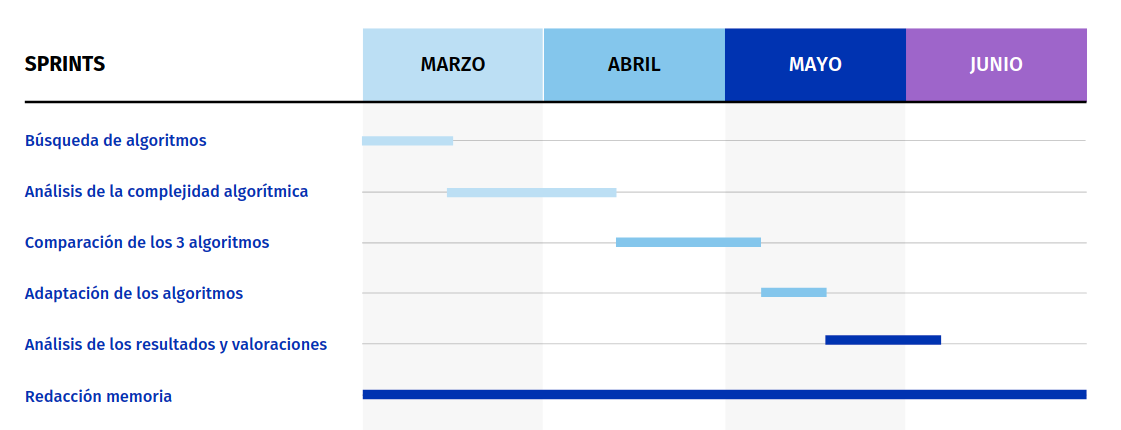
\includegraphics[width=1\textwidth]{imagenes/diagrama gantt.png} 
\end{center}

\section{Gestión de recursos}
En este sección se presentan los recursos tanto humanos, hardware y software que se han empleado para la elaboración del proyecto. 
\subsection{Recursos humanos}

\begin{itemize}
    \item \textbf{Tutora del proyecto}: Dña. Rocío Celeste Romero Zaliz, profesora de la Universidad de Granada del departamento de Ciencias de la Computación e Inteligencia Artificial
    \item \textbf{Alumno:} Francisco José Aparicio Martos, alumno de Ingeniería Informática de la Escuela Técnica Superior de Ingenierías Informática y Telecomunicaciones de la especialidad de Computación y Sistema Inteligentes.
\end{itemize}

\subsection{Recursos hardware}
Para la realización de este proyecto no se ha necesitado de recursos adicionales a los ya poseídos por el alumno. Todo el hardware ha sido aportado por el alumno siendo este:
\begin{itemize}
    \item \textbf{Portátil}: MSI GE63 Raider con un procesador intel core i7 de séptima generación y una tarjeta gráfica geforce gtx 1050 ti. Se ha usado en las labores de programación del proyecto, ejecución de pruebas y redacción de memoria.
    
    \item \textbf{Pantallas}: Dos pantallas, ASUS y SAMSUNG, de 24 pulgadas cada una.
\end{itemize}

\subsection{Recursos Software}
Todo el software empleado durante este proyecto es de uso gratuito englobándose gran parte en la categoría de software libre. A continuación se lista todo el software usado en el proyecto:

\begin{itemize}
    \item \textbf{Sistema Operativo}: Ubuntu Linux, versión 18.04.
    \item \textbf{Python}: más concretamente la versión 3.8.13, junto a python se usarán librerías incluidas en el propio python como por ejemplo: numpy y matplotlib, y librerías de uso libre que se encuentran subidas en la plataforma github. Más detalles sobre las librerías empleadas se puede encontrar en la sección de metodología.
    \item \textbf{Conda}: gestor de paquetes y de entornos para python.
    \item \textbf{Google Meet}: plataforma usada para realizar las reuniones por videollamada con la tutora.
    \item \textbf{Overleaf}: plataforma online para la redacción de documentos en \LaTeX.
    \item \textbf{Git}: software para el control de versiones. 
    \item \textbf{Github}: plataforma donde se alojará la memoria y el código del proyecto.
    \item \textbf{TimeCamp}: aplicación online para contabilizar cantidad de horas trabajadas.
\end{itemize}

\section{Presupuesto}
A continuación se presenta la estimación de los costes del proyecto teniendo en cuenta los recursos humanos, software y hardware presentados anteriormente. 

\subsection{Costes de recursos humanos}
En este apartado tenemos que incluir el coste del trabajo que he realizado.

Para realizar una estimación de cuanto costaría el trabajo realizado tenemos que ver cuál es el sueldo medio de un recién graduado en ingeniería informática. Según el portal jobted \footnote{\href{https://www.jobted.es/salario/ingeniero-informático}{Jobted}} el sueldo de un recién graduado en ingeniería informática gira entorno a los 20400 euros al año, por lo que si lo dividimos entre 12 meses, 20 días laborales por mes aproximadamente y 8 horas de jornada diaria, da como resultado un sueldo de 10.63 €/h. Teniendo en cuenta que las horas empleadas en el proyecto han sido 300 horas. Obtenemos que el coste de mi trabajo es de 3189 euros.


\subsection{Costes Software}
Como he comentado en el apartado de los recursos, todo el software que se ha usado en la elaboración de este proyecto es de uso gratuito por lo tanto estos recursos no añaden ningún tipo de coste al proyecto.

\subsection{Coste Hardware}
Los recursos hardware usados han sido mi ordenador y las pantallas que se han mencionado en la sección de recursos. Para calcular su valor hay que tener en cuenta que los productos electrónicos se devalúan con el paso de los años, para realizar este cálculo haremos uso del método de depreciación lineal, el cual nos indica cuanto valor pierde nuestro dispositivo por año.

\begin{equation}
    Depreciacion = \frac{valor\ inicial - valor\ residual}{vida\ util\ en\ a\tilde{n}os}
\end{equation}

Siendo el valor residual:
\begin{equation}
    Valor\ residual = \frac{valor\ inicial}{vida\ util\ en\ a\tilde{n}os}
\end{equation}

Este valor indica el valor final que tendrá el producto una vez llegue al fin de su vida útil. Para el caso de los dispositivos electrónicos la vida útil según la agencia tributaria española \footnote{\href{https://sede.agenciatributaria.gob.es/Sede/ayuda/manuales-videos-folletos/manuales-practicos/irpf-2019/capitulo-7-rendimientos-actividades-economicas-directa/fase-1-determinacion-rendimiento-neto/amortizaciones-dotaciones-ejercicio-fiscalmente-deducibles/requisitos-generales/coeficientes-amortizacion-lineal.html}{web agencia tributaria}} es de 10 años. Por lo tanto los valores actuales de cada uno de los dispositivos es de:

\begin{table}[H]
    \renewcommand{\arraystretch}{1.5}
    \centering
    \begin{tabular}{lcccc}
        \toprule[0.75mm]
        {\textbf{Recurso}} & \textbf{Valor inicial} & \textbf{Valor residual} & \textbf{Antigüedad} & \textbf{Valor actual}\\
        \hline
        Portátil & 1200€ & 120€ & 4 & 768€\\
        \hline
        Monitor Samsung & 190€ & 19€ & 2 & 155.8€\\
        \hline
        Monitor ASUS & 120€ & 12€ & 4 & 76.8€\\
        \bottomrule[0.75mm]
    \end{tabular}
    \caption{Tabla con los precios de los recursos hardware}
    %\label{tab:my_label}
\end{table}

\subsection{Presupuesto total}

Teniendo en cuenta todos los costes previamente calculados presento la siguiente tabla con el coste total del proyecto:
\begin{table}[H]
    \renewcommand{\arraystretch}{1.5}
    \centering
    \begin{tabular}{w{l}{6cm}w{r}{6cm}}
        \toprule[0.75mm]
        \textbf{Concepto} & \textbf{Importe}\\
        \hline
        \textbf{Recursos Hardware} & \\
        Portátil & 768€\\
        Monitor Samsung & 155.8€\\
        Monitor ASUS & 76.8€\\
        \hline
        \textbf{Recursos Humanos} & \\
        Trabajo individual & 3189€ \\
        \hline
        & \textbf{Total: 4189.6€} \\
        \bottomrule[0.75mm]
    \end{tabular}
    \caption{Presupuesto total del proyecto}
    %\label{tab:my_label}
\end{table}


\section{Análisis de riesgos}

Durante el desarrollo de cualquier proyecto siempre surgen imprevistos que alteran la programación inicial. Todos estos acontecimientos inesperados se conocen como riesgos. Para evitar que dichos riesgos afecten a la consecución de los objetivos, se deben de establecer una serie de protocolos a seguir con el objetivo de mitigar dichos problemas lo antes posible y conseguir que no afecten al trascurso del proyecto. Es por ello que antes de comenzar cualquier proyecto se debe de realizar una estimación acerca de los riesgos que pueden surgir y establecer planes de actuación. A continuación se presentan los riesgos que se han estudiado junto a sus causas y planes de actuación.


\begin{table}[H]
\centering
\begin{tabular}{|c|l|}
\hline
\rowcolor[HTML]{C0C0C0} 
{\color[HTML]{000000} \textbf{Código}} & {\color[HTML]{000000} \textbf{Riesgo}}                       \\ \hline
\rowcolor[HTML]{EFEFEF} 
{\color[HTML]{000000} 1} & {\color[HTML]{000000} No existe implementación de los algoritmos}           \\ \hline
\rowcolor[HTML]{EFEFEF} 
{\color[HTML]{000000} 2}               & {\color[HTML]{000000} No se encuentran alternativas viables} \\ \hline
\rowcolor[HTML]{EFEFEF} 
{\color[HTML]{000000} 3} & {\color[HTML]{000000} Las herramientas software no funcionan correctamente} \\ \hline
\rowcolor[HTML]{EFEFEF} 
{\color[HTML]{000000} 4}               & {\color[HTML]{000000} Incompatibilidad de librerías}         \\ \hline
\rowcolor[HTML]{EFEFEF} 
{\color[HTML]{000000} 5}               & {\color[HTML]{000000} No hay feed back del tutor}            \\ \hline
\rowcolor[HTML]{EFEFEF} 
{\color[HTML]{000000} 6}               & {\color[HTML]{000000} Pérdidas de código o datos}            \\ \hline
\rowcolor[HTML]{EFEFEF} 
{\color[HTML]{000000} 7}               & {\color[HTML]{000000} Se estropea el ordenador de trabajo}   \\ \hline
\end{tabular}
\caption{Tabla con los riesgos del proyecto}
\end{table}

\begin{table}[H]
\centering
\begin{tabular}{|c|l|}
\hline
\rowcolor[HTML]{C0C0C0} 
{\color[HTML]{000000} \textbf{Riesgo}} & {\color[HTML]{000000} \textbf{Causa}}                                \\ \hline
\rowcolor[HTML]{EFEFEF} 
{\color[HTML]{000000} 1}               & {\color[HTML]{000000} Los autores no han hecho públicos sus códigos} \\ \hline
\rowcolor[HTML]{EFEFEF} 
{\color[HTML]{000000} 2} & {\color[HTML]{000000} No se han realizado estudios que consigan resultados buenos}    \\ \hline
\rowcolor[HTML]{EFEFEF} 
{\color[HTML]{000000} 3}               & {\color[HTML]{000000} Bugs propios de los producto software}         \\ \hline
\rowcolor[HTML]{EFEFEF} 
{\color[HTML]{000000} 4} & {\color[HTML]{000000} Librerías que no se tenían pensadas para trabajar juntas}       \\ \hline
\rowcolor[HTML]{EFEFEF} 
{\color[HTML]{000000} 5} & {\color[HTML]{000000} No ha podido asistir a la reunión por incompatibilidad horaria} \\ \hline
\rowcolor[HTML]{EFEFEF} 
{\color[HTML]{000000} 6}               & {\color[HTML]{000000} Apagón repentino, fallo del almacenamiento}    \\ \hline
\rowcolor[HTML]{EFEFEF} 
{\color[HTML]{000000} 7}               & {\color[HTML]{000000} Sobrecalentamiento o golpe fortuito}           \\ \hline
\end{tabular}
\caption{Tabla con las causas de los riesgos}
\end{table}

\begin{table}[H]
\centering
\begin{tabular}{|c|l|}
\hline
\rowcolor[HTML]{C0C0C0} 
{\color[HTML]{000000} \textbf{Riesgo}} & {\color[HTML]{000000} \textbf{Plan de actuación}}                         \\ \hline
\rowcolor[HTML]{EFEFEF} 
{\color[HTML]{000000} 1} & {\color[HTML]{000000} Implementar el algoritmo a mano o de no ser posible buscar otra alternativa} \\ \hline
\rowcolor[HTML]{EFEFEF} 
{\color[HTML]{000000} 2}               & {\color[HTML]{000000} Probar con alternativas del propio backpropagation} \\ \hline
\rowcolor[HTML]{EFEFEF} 
{\color[HTML]{000000} 3}               & {\color[HTML]{000000} Buscar alternativa o corregir el error a mano}      \\ \hline
\rowcolor[HTML]{EFEFEF} 
{\color[HTML]{000000} 4}               & {\color[HTML]{000000} Buscar otro conjunto de librerías compatibles}      \\ \hline
\rowcolor[HTML]{EFEFEF} 
{\color[HTML]{000000} 5} & {\color[HTML]{000000} Planificar la reunión para otro día o mandar duda por correo}                \\ \hline
\rowcolor[HTML]{EFEFEF} 
{\color[HTML]{000000} 6}               & {\color[HTML]{000000} Recuperar datos a través del control de versiones}  \\ \hline
\rowcolor[HTML]{EFEFEF} 
{\color[HTML]{000000} 7}               & {\color[HTML]{000000} Comprar otro ordenador}                             \\ \hline
\end{tabular}
\caption{Tabla con los planes de actuación para cada riesgo}
\end{table}

\begin{table}[H]
\centering
\begin{tabular}{|
>{\columncolor[HTML]{EFEFEF}}l |
>{\columncolor[HTML]{67FD9A}}l |l|l|l|l|}
\hline
  \backslashbox{Impacto}{Probabilidad} &
  \cellcolor[HTML]{EFEFEF}0.1 &
  \cellcolor[HTML]{EFEFEF}0.3 &
  \cellcolor[HTML]{EFEFEF}0.5 &
  \cellcolor[HTML]{EFEFEF}0.7 &
  \cellcolor[HTML]{EFEFEF}0.9 \\ \hline
Muy bajo &
  {\color[HTML]{000000} } &
  \cellcolor[HTML]{67FD9A}{\color[HTML]{000000} R5} &
  \cellcolor[HTML]{67FD9A}{\color[HTML]{000000} } &
  \cellcolor[HTML]{FCFF2F}{\color[HTML]{000000} } &
  \cellcolor[HTML]{FCFF2F}{\color[HTML]{000000} } \\ \hline
Bajo &
  {\color[HTML]{000000} } &
  \cellcolor[HTML]{67FD9A}{\color[HTML]{000000} } &
  \cellcolor[HTML]{FCFF2F}{\color[HTML]{000000} } &
  \cellcolor[HTML]{FCFF2F}{\color[HTML]{000000} } &
  \cellcolor[HTML]{FFC702}{\color[HTML]{000000} } \\ \hline
Medio &
  {\color[HTML]{000000} } &
  \cellcolor[HTML]{FCFF2F}{\color[HTML]{000000} R3} &
  \cellcolor[HTML]{FCFF2F}{\color[HTML]{000000} R4} &
  \cellcolor[HTML]{FFC702}{\color[HTML]{000000} } &
  \cellcolor[HTML]{FFC702}{\color[HTML]{000000} } \\ \hline
Alto &
  \cellcolor[HTML]{FCFF2F}{\color[HTML]{000000} } &
  \cellcolor[HTML]{FCFF2F}{\color[HTML]{000000} R6} &
  \cellcolor[HTML]{FFC702}{\color[HTML]{000000} } &
  \cellcolor[HTML]{FFC702}{\color[HTML]{000000} } &
  \cellcolor[HTML]{FE0000}{\color[HTML]{000000} } \\ \hline
Muy alto &
  \cellcolor[HTML]{FCFF2F}{\color[HTML]{000000} R7} &
  \cellcolor[HTML]{FFC702}{\color[HTML]{000000} R2} &
  \cellcolor[HTML]{FFC702}{\color[HTML]{000000} R1} &
  \cellcolor[HTML]{FE0000}{\color[HTML]{000000} } &
  \cellcolor[HTML]{FE0000}{\color[HTML]{000000} } \\ \hline
\end{tabular}
\caption{Matriz probabilidad-impacto de riesgos}
\end{table}

